\documentclass[a4paper,12pt]{article}

\usepackage{cmap}                   
\usepackage{mathtext}   
\usepackage{mathtools}
\usepackage{amssymb,amsmath}
\usepackage{tipx}
\usepackage{tabularx,array,booktabs}
\usepackage{algorithm2e}
\usepackage{listings}
\usepackage{hyperref}
%изображения
\usepackage{graphicx}%Вставка картинок правильная
\usepackage{float}%"Плавающие" картинки
\usepackage{wrapfig}%Обтекание фигур (таблиц, картинок и прочего)
\usepackage{setspace}
\usepackage[normalem]{ulem}
\usepackage{arcs}
\usepackage[T1,T2A]{fontenc}        
\usepackage[utf8]{inputenc}         
\usepackage[english, russian]{babel} 
\usepackage[top=0.35in, bottom=0.5in, left=0.3in,right=0.3in]{geometry}
\usepackage{scalerel}
\usepackage{stackengine}
\stackMath
\newtheorem{theorem}{Теорема}
\newtheorem{definition}{Определение}
\newtheorem{proposal}{Предположение}
\newtheorem{notice}{Замечание}
\newtheorem{statement}{Положение}
\newtheorem{corollary}{Следствие}
\newtheorem{lemma}{Лемма}
\newtheorem{observation}{Наблюдение}
\newtheorem{problem}{Задача}
\newtheorem{claim}{Решение}

\newcommand{\RomanNumeralCaps}[1]
    {\MakeUppercase{\romannumeral #1}}
\newenvironment{shortlist}
  {\renewcommand{\item}{\renewcommand{\item}{\unskip\space\textbullet~}}}
  {}
\renewcommand{\tabularxcolumn}[1]{m{#1}}    
\newcommand\reallywidesmile[1]{%
\stackon[0.5pt]{#1}{%
\stretchto{%
  \scaleto{%
    \scalerel*[\widthof{#1}]{\mkern-1.5mu\smile\mkern-2mu}%
    {\rule[-\textheight/2]{1ex}{\textheight}}%
  }{\textheight}%
}{0.8ex}}%
}
\parskip 1ex


\title{Программирование в задачах радиолокации}
\author{КМБО-02-19}
\begin{document}

    \maketitle
    \section{ООП, принципы, отношения объектов}
\begin{notice}
Этот раздел - адаптация первой главы опросника по МиСП.
\end{notice}
\subsection{ООП}

    \begin{definition}
    \textbf{Объектно-ориентированный подход} - подход, при котором предметная область представлена совокупностью объектов, взаимодействующих между собой с помощью сообщений.
    \end{definition}
    
    \begin{definition}
    \textbf{Предметная область} - множество предметов и условий, в рамках которых происходит работа и выполнение задачи.
    \end{definition}
    \begin{definition}
    \textbf{Объект} - описание сущности из предметной области.
    \end{definition}
    \begin{definition}
    \textbf{Объектно-ориентированное программирование} - методология программирования, основанная на представлении программы в виде совокупности объектов.
    \end{definition}
    \begin{definition}
    \textbf{Класс} - множество объектов, обладающих общими свойствами и поведением.
    \end{definition}

\subsection{Свойства объекта}
    \begin{itemize}
        
        \item \begin{definition}\textbf{Состояние} - каждая уникальная комбинация свойств объекта(атрибутов) и связей с другими объектами. Меняется со временем.
        \end{definition}
        
        \item \begin{definition}\textbf{Поведение} - определяется методами - определяет действия объекта относительно внешних связей и манипуляций с собственными свойствами.
        \end{definition}
        
        \item \begin{definition}\textbf{Идентичность} - свойство объекта, отличающее его ото всех других объектов. \textit{В C++ это адрес}.
        \end{definition}
    \end{itemize}
    
\subsection{Принципы объектной модели}
\textbf{Основные принципы}:
\begin{itemize}
    \item \begin{definition}\textbf{Абстракция} - выделение наиболее существенных характеристик некоторого объекта, отличающих его от всех других объектов, важных с точки зрения дальнейшего рассмотртения.\end{definition}
    \item \begin{definition}\textbf{Инкапсуляция} - отделение друг от друга элементов объекта, определяющих его устройство и поведение. Служит для изоляции абстракции от реализации.\end{definition} 
    \item \begin{definition}\textbf{Модульность} - возможность спроектировать взаимодействия объектов так, чтобы объекты между собой взаимодействовали неинтенсивно, но внутри самих объектов происходила интенсивная работа. \textit{Используется для переиспользования объектов}.\end{definition}
    \item \begin{definition}\textbf{Иерархия} - упорядочивание абстракций по уровням.\end{definition}
\end{itemize}

\textbf{Дополнительные принципы}:
\begin{itemize}
    \item \begin{definition}\textbf{Типизация} - защита от неправильного использования объекта, т.е. от ситуации, когда объект одного класса используется вместо другого.\end{definition}
    \item \begin{definition}\textbf{Устойчивость} - возможность объекта переживать породивший его процесс.\end{definition}
    \item \begin{definition}\textbf{Параллелизм} - наличие в системе нескольких потоков управления одновременно.\end{definition}
\end{itemize}

\subsection{Принципы объектно-ориентированного программирования}
\subsubsection{Сами принципы}
\begin{enumerate}
    \item \textbf{Абстракция} - см. выше.
    \item \textbf{Инкапсуляция} - см. выше.
    \item \begin{definition}\textbf{Наследование} - механизм создания новых объектов на основе уже существующих путём сохранения свойств и поведения с возможностью расширения функциональности и переопределения.\end{definition}
    \item \begin{definition}\textbf{Полиморфизм} - возможность создавать объекты с одинаковым интерфесом и различной реализацией.\end{definition}
\end{enumerate}
\subsubsection{Примеры и особенности реализации принципов инкапсуляции, наследования и полиморфизма в C++}
\paragraph{Инкапсуляция} в C++ реализуется за счёт разделения атрибутов и методов класса(объекта) на публичные, защищённые и скрытые области видимости, реализующиеся с помощью спецификаторов public, protected и private соответственно.

$\qquad$ В листинге ниже представлен класс $Contact$, публичные переменные и методы доступны из основной программы $(main)$. Приватные переменные и методы могут прочитаны, вызваны или изменены только самим классом.Попытка напечатать или изменить приватную переменную $mobile\_number$ из основной программы $(main)$ вызовет ошибку при компиляции потому как доступ к приватным данным в классе ограничен.
\newpage
\lstset{language=C++, keepspaces = true, extendedchars=\false}
\lstinputlisting[language=C++]{encapsulation.cpp}
\newpage
\paragraph{Наследование} в C++ подразделяется на публичное$(public)$, защищённое$(protected)$ и приватное$(private)$.

Разница в следующем:
\begin{itemize}
    \item \textbf{Публичное наследование} - публичные и защищённые данные наследуются без изменения доступа к ним. Т.е. если в исходном классе было поле в защищённой области, то и для наследника это поле останется в защищённой области. Если у предка был публичный метод - он останется публичным и у наследника. 
    \item \textbf{Защищённое наследование} - все поля из public и protected родителя становятся protected-полями потомка.
    \item \textbf{Приватное наследование} - поля public и protected предка становятся полями private потомка.
\end{itemize}
\begin{notice}
    \textbf{Private поля предка ни в каком случае не наследуются!}
\end{notice}

Пример приватного наследования:
\lstset{language=C++}
\lstinputlisting[language=C++]{inheritance.cpp}

$\qquad$Класс $Computer$ теперь использует метод $turn\_on()$ как и любой приватный метод: $turn\_on()$ может быть вызван изнутри класса, но попытка вызвать его напрямую из $main$ приведет к ошибке во время компиляции. Для базового класса $Device$, метод $turn\_on()$ остался публичным, и может быть вызван из $main$.

\begin{notice}
    Более подробно о наследовании в C++, порядке вызовов конструкторов и деструкторов, виртуальном наследовании и прочем подробно написано в соответствующем разделе в материалах по \textit{методам и стандартам программирвания}. В этом же разделе приводятся лишь некоторые общетеоретические моменты.
\end{notice}

\paragraph{Полиморфизм} в C++ зачастую реализуется с помощью механизма наследования абстрактного класса классами с конкретной реализацией методов. Иными словами, существует \textbf{абстрактный класс - класс, в котором есть хотя бы одна чисто виртуальная функция} - от которого так или иначе наследуются другие классы, в которых как раз и создаётся реализация методов, заявленных в абстрактном классе. Также необходимо сказать о таких явлениях, как полиморфные функции: это некоторые функции, способные обрабатывать различные типы входных данных; наверняка Вы помните такие по первому семестру. Конечно, есть и другие проявления полиморфизма. 

\begin{notice}
В данном контексте мы говорим о так называемом \textbf{полиморфизме подтипов}(он же \textbf{Ad-hoc - полиморфизм}). Он заключается в том, что разным типам входных данных соответствует различное поведение.

Также различают так называемый \textbf{параметрический полиморфизм}, его суть в том, что для различных типов данных объект обеспечивает одинаковое поведение. Реализацию этого вида полиморфизма в C++ предлагает механизм шаблонов.

\end{notice}

$\qquad$ Для примера предлагаю рассмотреть нашу с вами лабораторную работу по написанию стека(её ведь все сделали, я надеюсь?). У нас есть абстрактный класс $StackImplementation$, содержащий интерфейс, который должна поддерживать структура, на основе которой работает стек. Уже от этого класса наследуются $VectorStack, ListStack$ - данные классы поддерживают уже реализации на конкретных структурах данных: векторе и списке соответственно. На следующей странице приведены примеры объявления класса $StackImplementation$ и класса $VectorStack$.
\newpage
\lstset{language=C++, keepspaces = true, extendedchars=\false}
\lstinputlisting[language=C++]{StackImplementation.h}
\lstset{language=C++, keepspaces = true, extendedchars=\false}
\lstinputlisting[language=C++]{VectorStack.h}

\newpage

\subsection{Типы отношений объектов}
\begin{definition}
    Отношения - способ организации взаимодействия.
\end{definition}

\subsection{Классификация:}
\begin{itemize}
    \item По виду: одно- и дву- направленные;
    \item По характеру: содержит (\textbf{has-a}), является (\textbf{is-a}), использует (\textbf{uses-a});
    \item По кратности: один на один, один объект на много объектов, много на много...
\end{itemize}

\begin{definition}
    \textbf{Интерфейс} - это контракт с системой, гарантирующий определённое поведение и свойства объекта.
\end{definition}

\subsubsection{Типы отношений:}
\begin{tabular}{|c|p{15cm}|}
\hline
     Зависимость& Она же может считаться конкретизацией поведения.
     Рассматривая на примере: один объект обращается к функции другого.
     При этом объекты \textbf{не являются полями друг друга}
     - отношение $(friend)$. Является однонаправленным отношением.
     \\
\hline
     Часть-целое& \begin{definition}
         \textbf{Агрегация} - целое не управляет жизненным циклом частей.
     \end{definition}
     Пример: работник переживает кампанию. Иными словами, если используем агрегацию, то в деструкторе агрегированный объект не удаляем. \textit{has-a}\\
     \cline{2-2}
     & \begin{definition}
         \textbf{Композиция} - часть принадлжеит только одному объекту, который за неё 'отвечает'.
     \end{definition} Пример: часть удаляется в деструкторе объекта-хозяина, а также находится в приватной части. \textit{has-a}\\
\hline
     Ассоциация& Объекты используют друг друга для своих нужд. Отношения двунаправленные, никто никому не принадлежит. Прекрасный пример: отношения врача и пациента - это явно не отношения часть-целое! У врача спокойно может быть огромное количество пациентов в день, а у пациента своя жизнь с блэкджеком и программированием в задачах радиолокации. \textit{uses-a}\\
\hline
     Наследование& Комментарии тут излишни, всё сказали раньше. \textit{is-a} \\
\hline
\end{tabular}
\begin{notice}
    Примеры на C++ для приведённых выше отношений объектов Вы без проблем можете придумать и сами. Поясним только следующее: пример \textbf{зависимости} мы можем найти, вспомнив класс $MyString$, где нам приходилось делать friend-ом класс 'ostream', чтобы работал корректный вывод; \textbf{часть-целое} - односвязный список - в идеале это композиция, ибо в деструкторе мы разрушаем все node в списке; наследование - очевидный пример со стеком; \textbf{агрегация} - возьмём какой-нибудь класс, который имеет полем $std::string$, получим, что класс не несёт ответственности за жизнь этого поля после себя, при этом это поле может быть передано и другим объектам; \textbf{ассоциация} - один класс запрашивает возвращаемые значения методов другого, чтобы конкретизировать свою работу - на пальцах сказать сложно, но если Вам попадётся код с такими отношениями, Вы сразу поймёте.
\end{notice}
\begin{notice}
    Если у Вас всё хорошо с английским и Вы не поняли того, что написано выше, предлагаю прочитать статью по ссылке:
    
    \url{https://www.learncpp.com/cpp-tutorial/10-1-object-relationships/}
\end{notice}

    \section{Структуры данных}

\begin{definition}
\textbf{Структура данных} - это формат организации данных, их управления и хранения, который обеспечивает эффективный доступ к ним и возможность их изменения.
\end{definition}

\begin{notice}
Из определения сразу понятно и назначение структур данных.
\end{notice}

По ссылке ниже Вы можете найти подробный гайд для понимания того, что такое структуры данных. По некоторым из тех структур, которые привёл автор, мы ещё поговорим в следующих разделах.

\url{https://habr.com/ru/post/310794/}
    \section{Вычислительная сложность алгоритмов. Пространственная и временная сложность}
\begin{notice}
    Далее я буду безбожно копипастить лекцию Макса по соответствующей теме, которая лежит в группе.
\end{notice}
\begin{definition}
    \textbf{Классический алгоритм} - конечная последовательность операций, понятная исполнителю, строгое исполнение которой решает поставленную задачу.
\end{definition}
\begin{notice}
    Также существуют специальные виды алгоритмов (например вероятностные), для которых не всегда определены перечисленные далее св-ва, но поставленную задачу они решают.
\end{notice}

\subsection{Свойства алгоритмов}

\begin{itemize}
    \item 
        \begin{definition}
            \textbf{Дискретность} - алгоритм должен представлять процесс решения задачи как последовательное выполнение некоторых простых шагов. При этом для выполнения каждого шага алгоритма требуется конечный отрезок времени, т.е. преобразование исходных данных в результат осуществляется во времени дискретно.
        \end{definition}
    \item
        \begin{definition}
            \textbf{Детерминированность} (определённость) - в каждый момент времени следующий шаг работы однозначно определяется состоянием системы. Таким образом, алгоритм выдаёт один и тот же результат для одних и тех же исходных данных.
        \end{definition}
    \item 
        \begin{definition}
            \textbf{Понятность} - алгоритм должен включать только те команды, которые доступны исполнителю и входят в его систему команд.
        \end{definition}
    \item 
        \begin{definition}
            \textbf{Конечность} - в более узком понимании алгоритма как математической функции, при правильно заданных начальных значениях алгоритм должен завершать работу и выдавать результат за определённое число шагов. Однако довольно часто определение алгоритма не включает завершаемость за конечное время.
        \end{definition}
    \item 
        \begin{definition}
            \textbf{Универсальность} - алгоритм должен быть применим к разным наборам начальных данных.
        \end{definition}
    \item 
        \begin{definition}
            \textbf{Результативность} - завершение алгоритма определёнными задачей результатами.
        \end{definition}
\end{itemize}

\subsection{Сложность алгоритма}
\begin{definition}
    \textbf{Вычислительная сложность - } функция зависимости ресурсов, затрачиваемых некоторым алгоритмом, от размера и состояния входных данных.
\end{definition}

Основными ресурсами являются:
\begin{itemize}
    \item Процессорное время (абстракция - время) 
    \item Память (абстракция - пространство)
\end{itemize}

\begin{notice}
    Когда идёт речь о сложности алгоритма, речь идёт не о конкретных величинах (секундах), а об абстрактных, таких, как количество элементарных операций.
\end{notice}

\begin{definition}
    \textbf{Принцип trade-off} - улучшение по сложности одного ресурса за счёт ухудшения по другому.
\end{definition}

При анализе сложности алгоритма можно рассматривать сложность:
\begin{itemize}
    \item в лучшем случае
    \item в среднем случае
    \item в худшем случае
\end{itemize}

\begin{definition}
    \textbf{Гарантированной сложностью} называется сложность алгоритма в худшем случае.
\end{definition}

\begin{definition}
    \textbf{Временная сложность} - функция от размера входных данных n, равная максимальному или среднему или минимальному количеству элементарных операций, проделываемых алгоритмом для решения экземпляра задачи.
\end{definition}
\begin{definition}
    \textbf{Пространственная сложность} - аналогично определению выше, но про объём памяти.
\end{definition}
    \section{Асимптотические и амортизационные оценки}
\begin{notice}
    Здесь мы попытаемся дать чуть более 'алгоритмический' материал, чем тот, что приведён в лекции.
\end{notice}

\begin{definition}
    \textbf{Асимптотическая оценка} - функция от времени, либо ограничивающая снизу $(\Omega(g(n)))$ или сверху $(O(g(n)))$ временную сложность алгоритма, либо совпадающая с ней$(\theta(g(n)))$.
\end{definition}

Нижние  оценки  позволяют  понять,  что  нельзя  реализовать  алгоритм эффективнее, чем полученная нижняя оценка.

Верхние оценки позволяют сделать вывод, что алгоритм будет работать не хуже, чем полученная нижняя оценка.

Оценки  одного  вида  различаются  по  «силе»:  очевидно,  что  для алгоритма с найденной верхней оценкой $O(n^4)$ семейство функций $O(n^{100})$ тоже будет являться  верхней  оценкой, но  эта  оценка  будет  являться  более слабой.

\begin{tabular}{|p{4.5cm}|p{2.5cm}|p{10cm}|}
    \hline
    \multicolumn{3}{|c|}{Наиболее распространённые значения $O$}\\
    \hline
     Имя&  Нотация&Пример, когда чаще возникает\\
    \hline
    Константная &$O(1)$ &Когда нет необходимости в трудоёмких операциях, таких как перенос данных, балансировка и проч. \textit{Пример:} вставка в связный список.\\
    \hline
    Логарифмическая &$O(log n)$ & Когда удаётся на каждом шаге алгоритма отсекать $\frac{n}{k}$ неподходящих вариантов. \textit{Пример:} бинарный поиск - худший случай(на каждом шаге отсекаем по половине от оставшегося массива), поиск в сбалансированном бинарном дереве (при переходе через один узел точно знаем, что одна из веток нам не подходит, т.е. каждый раз бракуем половинку от оставшихся данных).\\
    \hline
    Линейная &$O(n)$ & Когда необходимо проверить каждый элемент коллекции. Это либо цикл на отрезке $[0;n)$, либо эквивалентная ему рекурсия. \textit{Пример:} линейный обход неотсортированного массива для поиска минимума/максимума.\\
    \hline
    Линейно-логарифмическая &$O(n log n)$ & Возникает в ситуациях с вложенными циклами, в одном из которых можно сделать оптимизацию и постоянно отсевивать по половинке данных. \textit{Пример:} быстрая сортировка.\\
    \hline
    Полиноминальная &$O(n^2)$ & Cитуация вложенных циклов, каждый из которых честно отрабатывает на каждой своей итерации все элементы коллекции. \textit{Пример:} сортировка пузырьком.\\
    \hline
    Экспотенциальная &$O(2^n)$ & \textit{Пример:} алгоритмы перебора - \textit{brute force}.\\
    \hline
    Факториальная &$O(n!)$ & \textit{Пример:} неэффективные комбинаторные алгоритмы по поиску перестановок, размещений, сочетаний и проч.\\
    \hline
\end{tabular}

\subsection{Построение асимптотической оценки}
\begin{enumerate}
    \item Подсчитать максимальное количество элементарных операций, которые совершает алгоритм, в терминах $n$. Построить функцию $f(n)$ количества операций от времени.
    \item Оценить элементарные функции, входящие в $f(n)$: отбрасываем константы, константные множители, элементарные функции, которые являюются бесконечно малыми относительно других элементарных функций при $n \rightarrow \infty$.
    \item Радуемся результату.
\end{enumerate}

\textbf{Примеры на нахождение асимптотических оценок, после которых всё станет ясно:}

Рассмотрим следующий код:
\lstset{language=C++, keepspaces = true, extendedchars=\false}
\lstinputlisting[language=C++]{asympt.cpp}

Теперь предположим, что для процессора элементарными являются следующие операции:
\begin{itemize}
    \item Присваивание переменной значения;
    \item Доступ к элементу вектора по индексу;
    \item Сравнение двух чисел;
    \item Инкрементация значения;
    \item Основные арифметические операции.
\end{itemize}
Предположим также, что выбор между $if-else$ происходит мгновенно, время потребляет только проверка на выполняемость условия в $if$.

Теперь разберём код:
\begin{enumerate}
    \item В первой строке мы проводим 2 операции: получаем значение элемента по индексу, присваиваем его переменной - эти операции не зависят от $n$.
    \item Далее выражениям при заходе в цикл (инициализации $i = 0$, сравнению в выражении $i \textless n$) требуется по одной операции. Даже если $n = 0$, эти два выражения сожрут 2 операции.
    \item После захода в цикл каждую итерацию будем так или иначе иметь ещё по две операции: инкремент $++i$ и сравнение $i \textless n$ - они будут давать $+2$ на каждой итерации, $\Rightarrow$ от них будет $2n$ операций.
    \item Теперь получим некоторую функцию времени от входных данных $f(n) = 2n + 4$, где $4 = 2$ операции в первой строке $+ 2$ операции для инициализации цикла. 
    \item В теле цикла мы имеем сравнение в конструкции $if$, которое будет выполняться каждую итерацию, там же мы будем получать $i-ый$ элемента вектора$\Rightarrow$ имеем $+2n$ операций в цикле.
    \item Теперь встаёт вопрос о запуске тела условного оператора: в лучшем случае мы туда даже заходить не будем, в худшем - зайдём $n$ раз и получим каждый раз по 2 операции: вызом по индексу и присваивание, итого имеем $2n$.
    \item Теперь уточним $f(n)$: $f(n) = 4 + 2n + 2n + 0$ для лучшего случая и $f(n) = 4 + 2n + 2n + 2n$ для худшего случая.
\end{enumerate}
Теперь давайте разбираться с функцией в худшем случае:
\begin{enumerate}
    \item При анализе имеет значение только то, как себя ведут самые быстро растущие элементарные функции. Теперь смотрим на нашу: $f(n) = 6n + 4$ - константы при росте $n$ не растут $\Rightarrow$ избавляемся от них и получаем $f(n) = 6n$.
    \item Теперь откинем множитель перед оставшейся элементарной функцией. Себе объясним такую небрежность тем, что мы говорим об абстракции, а в реальности такие множители могут либо раздуваться, либо наоборот исчезать - всё зависит от используемого ЯП. Теперь имеем $f(n) = n$ и, следовательно, $O(f(n)) = O(n)$.
\end{enumerate}

\begin{notice}
    Как видно, мы оценивали здесь \textbf{худший случай}. При оценке лучшего случая, как нетрудно убедиться, мы получим ту же самую оценку, следовательно, можно даже заключить, что в этой ситуации мы имеем оценку времени алгоритма $\theta(n)$.
\end{notice}

Потренируемся находить асимптотики для следующих функций $f(n)$ (они же отображения $f: n\rightarrow t$):
\begin{enumerate}
    \item $f(n) = 5n + 12 \Rightarrow O(f(n)) = n$
    \item $f(n) = 109 \Rightarrow O(f(n)) = 1$ - здесь $109 = 109 * 1$, множитель убираем, а $1$ - элементарная функция наибольшего роста среди оставшихся.
    \item $f(n) = n^3 + 1999n + 1337 \Rightarrow O(f(n)) = n^3$ - если подходить нестрого, скажем, что в любом случае $n^3$ растёт быстрее линейной функции при стремлении к $\infty$. Но мы же математики, поэтому подойдём формально: \large{ $\lim_{n \to \infty} \frac{n^3}{199n} = \infty$}.
\end{enumerate}
Если всё-таки осталось что-то непонятое, рекомендую ознакомиться с этими статьями:

\url{https://habr.com/ru/post/173821/}

\url{https://habr.com/ru/post/196560/}

\subsection{Построение амортизационной оценки}
\begin{notice}
Здесь мы расскажем об алгоритме \textbf{группировки}(ещё называют алгоритмом агрегации). Помимо него есть \textbf{банковский алгоритм} и его обобщение - \textbf{метод потенциалов}. Последние два счастья в рунете изложены сложновато или не до конца полно, а искать на английском в 12 часов ночи уже не хочется.
\end{notice}

\textbf{Алгоритм группировки} состоит в следующем:
\begin{enumerate}
    \item Пусть $t_i$ - реальное время, потраченное на конкретную операцию. Тогда всего времени на $n$ операций было потрачено $\sum\limits_{i = 1}^n (t_i)$ времени.
    \item Теперь поймём, что $\sum\limits_{i = 1}^n (t_i) \geq n$, т.к. $\farall t_i \geq 1$.
    \item Наконец, получим амортизационную оценку: $amort(f(n)) = \frac{\sum\limits_{i = 1}^n (t_i)}{n}$
\end{enumerate}
Поясним на примере:
\begin{problem}
Необходимо найти амортизационную оценку для операции $push\_back$ в вектор, который мы реализовывали в течение семестра.
\end{problem}
\begin{claim}
    Начнём с такого наблюдения: пусть у нас есть изначально пустой вектор и в нём выделена память на 4 элемента.\\
    Первая, вторая, третья, четвёртая операции $push\_back$ выполнятся за $O(1)$. С пятой же операцией мы получим $O(n)$ - она же оценка худшего случая, т.к. в векторе произойдёт перевыделение памяти и перенос старых данных в новый контейнер.\\
    Теперь построим амортизационную оценку:
    $$
    \frac{1+1+1+1+n}{n} = \frac{4 + n}{n} = 1 + \frac{4}{n} \xrightarrow[n\rightarrow\infty]{}1\Rightarrow amort(O(f(n))) = amort(O(1))
    $$
\end{claim}






    \section{Массивы, векторы, связные списки. Устройство, основные операции, способы реализации}

\subsection{Массив}
\begin{definition}
    \textbf{Массив} - базовая структура данных - набор однотипных элементов, расположенных в памяти последовательно друг за другом.
\end{definition}
Пояснять тут больше нечего...

\subsection{Вектор}

\begin{definition}
    \textbf{Вектор} - структура данных, являющаяся надстройкой над массивом и поддерживающая следующие операции:
    \begin{itemize}
        \item Доступ к элементу; 
        \item Вставка элемента;
        \item Удаление элемента;
        \item Поиск.
    \end{itemize}
\end{definition}
\subsubsection{Устройство вектора}
Вектор содержит в себе динамический массив размера $capacity$. Текущее заполнение этого массива описывается параметром $size$.

Когда $size$ достигает определённого размера относительно $capacity$(об этом поговорим чуть позже), происходит перевыделение памяти: либо выделяется блок памяти размером поменьше, либо размером побольше - и туда перемещается $size$ элементов массива. Одновременно с этим меняется и $capacity$.

\subsubsection{Изменение $capacity$ в векторе}
Существует две стратегии изменения $capacity$:
\begin{itemize}
    \item Аддитивная: $capacity = oldCapacity + \Delta$. При этом $\Delta$ задаётся либо по умолчанию, либо в момент создания вектора.
    \item Мультипликативная: $capacity = coef * oldCapacity$. При этом $coef$ задаётся либо по умолчанию, либо в момент создания вектора.
\end{itemize}

\subsubsection{Условие изменения $capacity$ в векторе}
Здесь вволится следующая величина:
$$
loadFactor = \frac{size}{capacity}
$$
\begin{equation*}

\textbf{Если выбрана аддитивная стратегия:}

    \begin{cases}
        if (loadFactor \geq 0.8) \Rightarrow while(loadFactor \geq 0.8) capacity := capacity + \Delta;
    \end{cases}
    
\textbf{Если выбрана мультипликативная стратегия:}

    \begin{cases}
    if (loadFactor \leq \frac{1}{coef^2}) \Rightarrow \text{обрезаем память} \\
    if (loadFactor \geq 0.8) \Rightarrow \text{Перевыделяем память}\\
    \end{cases}
\end{equation*}

\subsubsection{Оценки операций с вектором}
\begin{tabular}{|p{2.5cm}|p{3.5cm}|p{3.5cm}|p{3.5cm}|}
\hline
     & Лучший случай & Средний случай&Худший случай \\
\hline
    Доступ & $O(1)$ & $O(1)$ & $O(1)$\\
\hline
    Вставка & $Amort(O(1))$ [вставка в конец]& $O(n)$ [вставка не в конец] & $O(n)$  [вставка в начало]\\
\hline
    Удаление & $Amort(O(1))$ [удаление с конца]& $O(n)$ [удаление не из конца]& $O(n)$ [удаление первого элемента]\\
\hline
    Поиск & $O(1)[искомый - первый]$ & $O(n)$ [искомый - не первый] & $O(n)$ [искомый - последний]\\
\hline
\end{tabular}
\subsubsection{Резюме}
\begin{tabular}{cp{10cm}}
    Достоинства: &
        \begin{equation*}
            \begin{cases}
                \text{Минимальный } overhead;\\
                \text{Простота реализации};\\
                \text{Быстрый доступ к элементам коллекции}.
            \end{cases}
        \end{equation*} \\
    Недостатки:&  
        \begin{equation*}
            \begin{cases}
                \text{Необходимо иметь нефрагментированную память;}\\
                \text{При большой загрузке долгое перевыделение памяти.}\\
            \end{cases}
        \end{equation*} 
\end{tabular}

\textbf{Используется в задачах, где необходим \textit{гарантированно} быстрый доступ к данным}.
\newpage
\subsection{Связный список}
\begin{definition}
    \textbf{Связный список} - структура данных, в которой каждый элемента содержит указатель на следующий элемент (случай односвязного списка) или и на следующий, и на предыдущий (двусвязный список).
\end{definition}

\begin{figure}[ht]
    \centering
    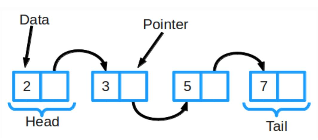
\includegraphics[scale=1]{List.png}
    \caption{Односвязный список}
    \label{fig:g}
\end{figure}

\subsubsection{Основные операции над списками}
\begin{itemize}
        \item Доступ к элементу; 
        \item Вставка элемента;
        \item Удаление элемента;
        \item Поиск.
\end{itemize}

\subsubsection{Оценка операций}
\begin{tabular}{|p{3cm}|p{3cm}|p{3cm}|p{3cm}|}
\hline
     & Лучший случай & Средний случай&Худший случай \\
\hline
    Доступ & $O(1)$ & $O(n)$ & $O(n)$\\
\hline
    Вставка (\textbf{если знаем}, куда вставлять) & $O(1)$ [вставка в конец]& $O(1)$  & $O(1)$  \\
\hline
    Удаление (\textbf{если знаем}, откуда удалять) & $O(1)$ & $O(1)$ & $O(1)$\\
\hline
    Поиск & $O(1)[искомый - первый]$ & $O(n)$ [искомый - не первый] & $O(n)$ [искомый - последний]\\
\hline
\end{tabular}

\subsection{Резюме}
\begin{tabular}{cp{10cm}}
    Достоинства: &
        \begin{equation*}
            \begin{cases}
                \text{Быстрое удаление};\\
                \text{Быстрая вставка};\\
                \text{Нет ограничений на фрагментацию памяти}.
            \end{cases}
        \end{equation*} \\
    Недостатки:&  
        \begin{equation*}
            \begin{cases}
                \text{Довольно приличный }overhead;\\
                \text{Долгий доступ к элементая коллекции.}\\
            \end{cases}
        \end{equation*} 
\end{tabular}

\textbf{Используется в задачах, где необходимы \textit{гарантированно} быстрые добавление и удаление узлов}.
\end{document}
